\documentclass[]{article}
\usepackage{fancyvrb}
\usepackage{amsmath}\usepackage{amsfonts}
\usepackage[margin=1in,footskip=0.25in]{geometry}
\usepackage{mathtools}
\usepackage{hyperref}
\hypersetup{
    colorlinks=true,
    linkcolor=blue,
    filecolor=magenta,
    urlcolor=cyan,
}
\usepackage[final]{graphicx}
\usepackage{listings}
\usepackage{courier}

\lstset{basicstyle=\footnotesize\ttfamily,breaklines=true}
\newcommand{\indep}{\perp \!\!\! \perp}
% \usepackage{wrapfig}
\graphicspath{{.}}
\begin{document}
\begin{center}
    Name: Hongda Li
    \\
    AMATH 516 HW4 2021 FALL 
\end{center}
\section*{4.2}
    This is the Fenchel Rockafella Primal Dual Problems: 
    \begin{align*}\tag{4.2.1}\label{eqn:4.2.1}
        (P)& \inf_{x\in \mathbf{E}} \left\lbrace
            h(\mathcal{A}x) + g(x)
        \right\rbrace
        \\
        (D) & \sup_{y \in \mathbf{Y}} \left\lbrace
            - h^{\star} - g^\star(-\mathcal{A}^*y)
        \right\rbrace
    \end{align*}
    Where we use $\star$ for the Fenchel Conjugate of the function and $*$ for adjoint operator. 
    \\
    Sometimes we need to take the subdifferential/gradient/conjugate of an expression involving multiple parameters, we denote it as the following: 
    $$
        \nabla [f(x, y)| x] 
        \quad
        \partial [f(x, y)|x]
        \quad 
        [f(x, y)| x]^\star
    $$
    Where the bar notation is telling use which variable we are taking the derivative wrt to the parameter. 
    \subsection*{4.2.1}
        We wish to compute the Fenchel Rockafella's Dual for the following Optimization Problem: 
        $$
            \min_{x} \left\lbrace
                \frac{1}{2}\left\Vert
                     Ax - b
                \right\Vert_2^2 + \Vert x\Vert_1
            \right\rbrace
        $$
        To compute the Dual first identify $f, g$: 
        \begin{align*}\tag{4.2.1.1}\label{eqn:4.2.1.1}
            h(Ax) &= \frac{1}{2}\Vert Ax - b\Vert_2^2 
            \\
            \implies h(x) &= \frac{1}{2}\Vert x - b\Vert_2^2
            \\
            g(x) &= \Vert x \Vert_1
        \end{align*}
        Considering the Fenchel Conjugate of $h(x)$: 
        \begin{align*}\tag{4.2.1.2}\label{eqn:4.2.1.2}
            h^\star(x) &= \sup_{y} \left\lbrace
                \left\langle x, y \right\rangle - h(y)
            \right\rbrace
            \\
            &= \sup_{y} \left\lbrace
                \left\langle x, y \right\rangle - 
                \frac{1}{2}\left\Vert
                    y - b
                \right\Vert_2^2
            \right\rbrace
            \\
            \partial\left[
                \left.
                    \left\langle x, y \right\rangle 
                    -
                    \frac{1}{2} \Vert y - b\Vert_2^2
                \right| y
                \right] &= \{x - (y - b)\}
            \\
            0 &\in \{x - (y^+ - b)\}
            \\
            \implies
            y^+ &= x + b
            \\
            \implies 
            h^\star(x) &= \langle 
            x, x + b
            \rangle - \frac{1}{2}\left\Vert
                x
            \right\Vert_2^2
            \\
            &= 
            \langle x, x\rangle + \langle x, b\rangle - 
            \frac{1}{2}\left\Vert
                x
            \right\Vert_2^2
            \\
            &= 
            \Vert x\Vert_2^2 + \langle x, b\rangle - 
            \frac{1}{2}\left\Vert
                x
            \right\Vert_2^2
            \\
            h^\star(x)
            &= \frac{1}{2}\Vert x\Vert_2^2 + \left\langle 
                x, b
            \right\rangle
        \end{align*}
    In this case, the function is continuous and it's concave, therefore a minimum eixsts and if I take the derivative and set it zero, I can get the optimal paramter $y^+$ and find the supremum. 
    \\
    Next we compute the Conjugate for $g(x)$: 
    \begin{align*}\tag{4.2.1.3}\label{eqn:4.2.1.3}
        g(x) &= \Vert x\Vert_1
        \\
        g^\star(x) &= 
        \sup_{y} \left\langle 
            \left\langle x, y \right\rangle - \Vert y\Vert_1
        \right\rangle
        \\
        &= 
        \sup_y \left\lbrace 
            \sum_{i = 1}^{n} (x_iy_i - |y_i|)
        \right\rbrace
        \\
        &= 
        \sum_{i = 1}^{n} \sup_{y_i} \left\lbrace
            x_iy_i - |y_i|
        \right\rbrace
    \end{align*}
    The sup can goes in because it's a summing up discrate expression each using $y_i$, and we assume that $y\in \mathbb{R}^n$, and we can say that:
    \begin{align*}\tag{4.2.1.4}\label{eqn:4.2.1.4}
        \forall 1 \le i \le n & 
        \\
        \sup_{y_i} \left\lbrace
            x_i y_i - |y_i|
        \right\rbrace &= 
        \max\left\lbrace
            \sup_{y_i \ge 0}\left\lbrace
                x_i y_i - y_i
            \right\rbrace, 
            \sup_{y_i < 0}\left\lbrace
                x_i y_i + y_i
            \right\rbrace
        \right\rbrace
        \\
        \sup_{y_i> 0} \left\lbrace
            y_i(x_i - 1)
        \right\rbrace &= 
        \begin{cases}
            \infty & x_i > 1 
            \\
            0 & x_i \le 1
        \end{cases}
        \\
        \sup_{y_i < 0}\left\lbrace
                y_i(x_i + 1)
        \right\rbrace
        &= 
        \begin{cases}
            0 & x_i \ge - 1
            \\
            \infty & x_i < -1
        \end{cases}
        \\
        \implies
        \forall 1 \le i \le n 
        \quad
        \sup_{y_i} \left\lbrace
            x_i y_i - |y_i|
        \right\rbrace &=
        \begin{cases}
            0 &|x_i| \le 1
            \\
            \infty & |x_i| > 1
        \end{cases}
        \\
        \implies
        \sum_{i = 1}^{n} \sup_{y_i} \left\lbrace
            x_iy_i - |y_i|
        \right\rbrace
        &= \begin{cases}
            \infty & \Vert x\Vert_\infty > 1
            \\
            0 & \Vert x\Vert_\infty \le 1
        \end{cases}
        \\
        \implies
        g^\star(x) &= \delta\{\Vert x\Vert_\infty \le 1\}(x)
    \end{align*}
    The conjugate of $g$ is the indicator function of the unit infinity norm ball. 
    \\
    Now we are ready to use the conjugate function to figure out the Fenchel Rockafella's Dual, we use the results from \hyperref[eqn:4.2.1.2]{(4.2.1.2)} and \hyperref[eqn:4.2.1.4]{(4.2.1.4)}: 
    \begin{align*}\tag{4.2.1.5}\label{eqn:4.2.1.5}
        & \sup_{y} \left\lbrace
            -h^\star(y) - g^\star(- \mathcal{A}^*y)
        \right\rbrace
        \\
        \equiv & \sup_{y} \left\lbrace
            - \frac{1}{2}\Vert y\Vert_2^2 - \langle y, b\rangle - 
            \delta\{\Vert -A^Ty\Vert_\infty \le 1\}(x)
        \right\rbrace
        \\
        \equiv&
        \sup_{\Vert A^Ty\Vert_\infty \le 1} \left\lbrace
            - \frac{1}{2}\Vert x\Vert_2^2 - \langle x, b\rangle
        \right\rbrace
    \end{align*}
    \subsection*{4.2.2}
        We wish to look for the Dual for the following problem: 
        $$
            \min_{\Vert x\Vert_q \le 1} \Vert Ax - b\Vert_p
        $$
        Where we are going to use $\Vert x \Vert_m, \Vert x\Vert_{\bar{m}}$ to denote the norm and its dual norm. First we identify the $f, g$ as: 
        \begin{align*}\tag{4.2.2.1}\label{eqn:4.2.2.1}
            h(x) & = \Vert x - b\Vert_p 
            \\
            g(x) &= \delta \{\Vert x\Vert_q\le 1\}(x)
        \end{align*}
        Before we start I am going to introduce a convenient new trick and I am going to prove it: 
        \\
        \textbf{Claim}:
         ``Conjugate of a Norm is the indicator function for the unit norm ball of the Dual Norm.''
        \\
        \textbf{Proof}:\\
        Set $f(x) = \Vert x\Vert$ and we use $\Vert x\Vert_*$ to denote the dual norm, and we wish to prove that $f^\star(x) = \delta \{\Vert x\Vert_* \le 1\}(x)$. Recall that the definition of dual norm is: 
        $$
            \Vert y\Vert_* = \sup_{\Vert x\Vert\le 1}\left\langle x , y \right\rangle
        $$
        From the definition of the conjugate of a function we have: $f^\star(x) = \sup_y \{\langle x, y\rangle - f(y)\}$, and let's discuss it by cases: 
        \\
        Suppose that $\Vert y\Vert_* \le 1$ then: 
        \begin{align*}\tag{4.2.2.2}\label{eqn:4.2.2.2}
            1 \ge \Vert y\Vert_* &\ge \sup_{\Vert x\Vert \le 1}\{\langle x, y\rangle\}
            \\ 
            \forall \Vert x\Vert \le 1 : \; & \langle x, y\rangle \le 1 
            \\
            \text{let: } t &> 0
            \\
            \langle tx, y\rangle &\le t \langle x, y\rangle \le t = t \Vert x\Vert = \Vert t x\Vert
            \\
            \implies 
            \forall\; tx \; , \Vert x\Vert \le 1: \langle tx, y\rangle &\le \Vert t  x\Vert
            \\
            \implies 
            \forall x \; \langle x, y\rangle &\le \Vert x\Vert
            \\
            \implies \sup_x \{\langle y, x\rangle - \Vert x\Vert\} &=  0
        \end{align*}
        Because the inner produce is forever smaller than the norm of $x$, therefore we have to set the value of $x = 0$ to attain the sup of the expression, which is zero. 
        \\[1.1em]
        Next we consider the case where $\Vert y\Vert_* > 1$, and we can say that: 
        \begin{align*}\tag{4.2.2.3}\label{eqn:4.2.2.3}
            \Vert y\Vert_* & > 1
            \\
            \exists x: \; \Vert x\Vert &\le 1 \wedge \langle x, y\rangle > 1 
            \\
            \implies 
            \sup_y \{\langle x, y \rangle   - \Vert x\Vert\} &\ge 
            \langle x, y \rangle - \Vert x\Vert > 0 
            \\
            \text{let } x &= tx, t \ge 0 
            \\
            t \langle x, y \rangle - t \Vert  x\Vert &> 0 
            \\
            t(\langle x, y \rangle - \Vert x\Vert) &> 0
            \\
            \implies \sup_y \{\langle x, y \rangle - \Vert x\Vert\} &= \infty
        \end{align*}
        Therefore the conjugate of the function $f$ is: $f^\star(x) = \delta \{\Vert x\Vert_* \le 1\}(x)$. It's the indicator function of the dual unit norm ball. 
        \\[1.1em]
        Using this pieces of information, we can start figuring out the conjugate. From table 3.4 and the fact that the function $f, h$  are both norm of something, hence convex, therefore the double conjugate of the function is the funciton itself. Therefore the table can be applied in both forward and backwards direction. In our case, we are applying the seceond entry of table 3.4. 
        \begin{align*}\tag{4.2.2.4}\label{eqn:4.2.2.4}
            \left[
                \left . f(x + b) \right| x
            \right]^\star &= 
            f^\star(y) - \langle b, y\rangle
        \end{align*}
        In our case we have: 
        \begin{align*}\tag{4.2.2.5}\label{eqn:4.2.2.5}
            \left[
                \left. \Vert x - b\Vert_p 
                \right| 
                x
            \right]^\star (y) 
            &= 
            \delta \{\Vert x\Vert_{\bar{p}} \le 1\}(y)  - \langle b, y \rangle
        \end{align*} 
        By a similar token the conjugate of the $g$ function would be: 
        \begin{align*}\tag{4.2.2.6}\label{eqn:4.2.2.6}
            \left[
                \delta \{
                    \Vert x\Vert_{q \le 1}(x)
                \}
            \right]^\star(y) &= \Vert y\Vert_{\bar{q}}
        \end{align*}
        Results are out: 
        $$
            h(x) = \Vert x - b\Vert_p \quad g(x) = \delta \{\Vert q\Vert \le 1\}(x)
        $$
        And using the Rockafella's Duality we have: 
        \begin{align*}\tag{4.2.2.7}\label{eqn:4.2.2.7}
            \sup_{\Vert y\Vert_{\bar{p}}\le 1} 
            \left\lbrace
                \left\langle b, y \right\rangle - \Vert A^Ty\Vert_{\bar{q}}
            \right\rbrace
        \end{align*}
        The negative sign can get ignore because $g^\star$ is a norm. 
    \subsubsection*{4.2.3}
        The primal is: 
        $$
            (P): \min_x\left\lbrace
                \left\langle c, x \right\rangle: Ax = b, x \in K
            \right\rbrace
        $$
        Where $K$ is a cone. 
        \\
        Identifies the $g, h$ function in this case it's: 
        \begin{align*}\tag{4.2.3.1}\label{eqn:4.2.3.1}
            h(Ax) &= \delta \{Ax = b \} 
            \\
            \implies h(x) &= \delta \{x = b\}
            \\
            g(x) &= \langle c, x\rangle + \delta \{x \in K\}
        \end{align*}
        We can immdiately identifies the conjugate of the indicator function $h$ because it's part of the Exercise 3.24 from the last homework. And therefore we have: $h^\star(x) = \langle b, x\rangle$. 
        \\
        To figure out the Conjugate of $h$: 
        \begin{align*}\tag{4.2.3.2}\label{eqn:4.2.3.2}
            g^\star(x) &= \sup \{\langle x, y \rangle - g(y)\}
            \\
            &= \sup_y \{
                \left\langle x, y \right\rangle - \left\langle c, y \right\rangle - \delta\{y \in K\}(y)
            \}
            \\
            &= \sup_y \{
                \left\langle y, x - c \right\rangle - \delta\{y \in K\}(y)
            \}
            \\
            &= \sup_{y\in K}\{\left\langle y, x- c \right\rangle\}
            \\
            &= \delta^\star_{K}(x - c)
        \end{align*}
        Using page 60 of the textbook, and the fact that $K$ is a cone, we have: $g^\star(x) = \delta^\star_K(x - c) = \delta_{K^\circ}(x - c)$. 
        \\
        The Fenchel Dual is: 
        \begin{align*}\tag{4.2.3.3}\label{eqn:4.2.3.3}
            \sup_{y} \left\lbrace
                - h^{\star}(y) - g^\star(- A^*y)
            \right\rbrace
            &= 
            \sup_{y} \left\lbrace
                - \left\langle b, y \right\rangle - \delta_{K^\circ} (-A^Ty - c)
            \right\rbrace
            \\
            &\equiv 
            \sup_{y} \left\lbrace
                \left\langle b, y \right\rangle - \delta_{K^\circ} (A^Ty - c)
            \right\rbrace
        \end{align*}
    \subsection*{4.2.4}
        The Primal Problem is: 
        $$
            (P): \min_{x} \left\lbrace
                \frac{1}{2} \left\langle x, Qx \right\rangle + \left\langle c, x \right\rangle: Ax \le b
            \right\rbrace
        $$
        Where the matrix $Q$ is Positive Definite. Identifying the $g, h$ we have: 
        \begin{align*}\tag{4.2.4.1}\label{eqn:4.2.4.1}
            h(Ax) &= \delta \{Ax \ge b \}(x)
            \\
            g(x) &= \frac{1}{2}\Vert x\Vert_Q^2 + \left\langle x, c \right\rangle
            \\
            \implies h(x) &= 
            \delta\{x \ge b\}(x)
            \\
            &= \delta\{x - b \ge 0\}(x)
        \end{align*}
        Notice that $x - b\ge 0 \iff x - b \in \mathbb{R}_+^n$ and $\mathbb{R}_+^n$ is a cone and it's polar cone is $\mathbb{R}^n_-$. Therefore, we use table 3.4: 
        \begin{align*}\tag{4.2.4.2}\label{eqn:4.2.4.2}
            h(x) &= \delta_{\mathbb{R}_+^n}(x -b)
            \\
            \implies h(x + b) &= \delta_{\mathbb{R}_+^n}(x)
            \\
            \implies
            h^\star(x) &= \delta_{\mathbb{R}_-^n}(x) - \left\langle b, x \right\rangle
        \end{align*}
        The conjugate of $g$ is given by: 
        \begin{align*}\tag{4.2.4.3}\label{eqn:4.2.4.3}
            g^\star(y) &= 
            \left[
                \left.
                    \frac{1}{2}\Vert x\Vert_Q^2 + \left\langle c, x \right\rangle
                \right| x
            \right]^\star (y)
            \\
            &=  
            \left[
                \left.
                    \frac{1}{2}\Vert x\Vert_Q^2
                \right| x
            \right]^\star (y- c)
        \end{align*}
        Let's figure out the conjugate of the one half of the Energy Norm squared: 
        \begin{align*}\tag{4.2.4.4}\label{eqn:4.2.4.4}
            \left[
                \frac{1}{2} \Vert A^{1/2}x\Vert_2^2
            \right]^\star(y) &= 
            \sup_{x} \left\lbrace
                \langle y, x\rangle - \frac{1}{2} \Vert A^{1/2}x\Vert_2^2
            \right\rbrace
            \\
            \text{Set Gradient to zero to find the sup}& 
            \\
            \nabla \left[
                \left.
                    \langle y, x\rangle - \frac{1}{2}\Vert x\Vert_A^2
                \right|x
            \right] &= 0
            \\
            \implies y - Ax^+ &= 0
            \\
            Ax^+ &= y
            \\
            x^+&= A^{-1}y
            \\
            \implies
            \sup_{x} \left\lbrace
                \langle y, x\rangle - \frac{1}{2} \Vert A^{1/2}x\Vert_2^2
            \right\rbrace &= 
            \langle y, A^{-1}y\rangle - \frac{1}{2}\Vert A^{-1/2}y\Vert_2^2
            \\
            &= 
            \Vert y\Vert_{A^{-1}}^2 - \frac{1}{2}\Vert y\Vert_{A^{-1}}^2
            \\
            &= 
            \frac{1}{2}\Vert y\Vert_{A^{-1}}^2
        \end{align*}
        Then we can conclude together with the results from \hyperref[eqn:4.2.4.3]{(4.2.4.3)} to get: 
        \begin{align*}\tag{4.2.4.5}\label{eqn:4.2.4.5}
            g^\star(y)  &= \frac{1}{2} \Vert y - c\Vert_{Q^{-1}}^2
        \end{align*}
        Therefore, the Dual is: 
        \begin{align*}\tag{4.2.4.6}\label{eqn:4.2.4.6}
            \max_{y}\left\lbrace
                - h^\star(y) - g^\star(-\mathcal{A}^*y)
            \right\rbrace
            &=
            \max_{y} \left\lbrace
                \delta_{\mathbb{R}_-^n}(y) - \langle b, y\rangle - \frac{1}{2} \Vert -A^Ty - c\Vert_{Q^{-1}}^2
            \right\rbrace
            \\
            &\equiv 
            \max_{y \ge 0} \left\lbrace
                \left\langle b, y \right\rangle - \frac{1}{2}\Vert A^Ty - c\Vert_{Q^{-1}}^2
            \right\rbrace
        \end{align*}
\section*{5.14}
    For this part of the HW I implemented the Smooth Gradient Descend and the Accelerated Gradient on Julia the programming language and made the plot of for the values of the objective functions for the first 100 iterations of both method. (Running the code requires installing UnicodePlots.jl and Plots.jl)
    \\
    This is how I got the gradient for the function for the implementations. 
    \\
    Let $X\in \mathbb{R}^{m\times n}$, let $y\in \mathbb{R}^m$, $\theta \in \mathbb{R}^n$. And let lower case $x_i$ denotes the $i$ th of the matrix $X$ The Gradient of the loss function is computed as: 
    \begin{align*}\tag{5.14.1}\label{eqn:5.14.1}
        & \nabla_\theta \left[
            \sum_{i = 1}^{m}\ln(1 + \exp \left(
                \langle \theta, -y_ix_i)\rangle
            \right)) + \frac{\lambda}{2}\Vert \theta\Vert_2^2
        \right]
        \\
        &= 
        \left(
            \sum_{i = 1}^{m}
            \nabla_\theta \left[
                \ln\left(
                    1 + \exp \langle \theta, -y_i x_i\rangle
                \right)
            \right]    
        \right) + \lambda\theta
        \\
        &= \left(
            \sum_{i = 1}^{m}\frac{
                \exp(\theta, -y x_i)
            }{1 + \exp(\theta, -y x_i)}
            \nabla_\theta[
                \langle \theta, -y_ix_i\rangle
            ] 
        \right) + \lambda \theta
        \\
        &= 
        \left(
            \sum_{i = 1}^{m}\frac{
                -\exp(\theta, -y x_i)
            }{1 + \exp(\theta, -y x_i)}
            yx_i
        \right) + \lambda \theta
    \end{align*}
    The code implementations is here: 
    \begin{Verbatim}[numbers=left]
using LinearAlgebra
import UnicodePlots
import Plots
import Logging

# ------------------------------------------------------------------------------
mutable struct LogisticRegressionModel
    X::Matrix{Float64}       # The data
    y::Vector{Float64}       # the labels
    theta::Vector{Float64}   # The parameters
    lambda::Float64          # a regularization parameters
    
    function LogisticRegressionModel(X, y, theta; lambda=1)
        this = new(X, y, theta, lambda)
        return this
    end

end

function Base.copy(this::LogisticRegressionModel)
    return LogisticRegressionModel(
        copy(this.X),
        copy(this.y), 
        copy(this.theta), 
        lambda = copy(this.lambda)
        )
end

function ErrorOf(this::LogisticRegressionModel)
    theta = this.theta
    X = this.X
    y = this.y
    lambda = this.lambda

    Error = - y.*(X*theta)  # vector 
    Error = 1 .+ exp.(Error)  # vector
    Error .= log.(Error)  # vector
    Error = sum(Error)
    Error += (lambda/2)*dot(theta, theta)
    return Error
end

function GradientOf(this::LogisticRegressionModel)
    theta = this.theta
    X = this.X
    y = this.y
    lambda = this.lambda

    Expr1 = (x) -> exp(x)/(1 + exp(x))
    Summation = zeros(size(theta))
    for Index = 1:size(X, 1)
        x = X[Index, :]
        Expr2 = - y[Index]*x  # vector
        Expr3 = dot(theta, Expr2)  # scalar
        Summation += Expr1(Expr3) * Expr2  # Vector
    end
    # ----------------------------------------------
    # Summation = exp.(-y.*X*theta)
    # Summation = Summation./(Summation .+ 1)
    # Summation = X'*(-y.*Summation)
    return Summation + lambda*theta
end

function ParametersOf(this::LogisticRegressionModel)
    return this.theta
end



# ------------------------------------------------------------------------------
mutable struct GradientDescend
    beta::Float64
    objective::LogisticRegressionModel
    objective_vals::Vector{Float64}
    
    function GradientDescend(objective::LogisticRegressionModel, beta::Float64)
        this = new(beta, objective, Vector{Float64}())
        push!(this.objective_vals, ErrorOf(this.objective))  # initial error. 
        return this
    end
end


function GradientUpdate(this::GradientDescend)
    DeltaTheta = GradientOf(this.objective)
    Params = ParametersOf(this.objective)
    Params .-= DeltaTheta * (1/this.beta)
    push!(this.objective_vals, ErrorOf(this.objective))
    
    return norm(DeltaTheta)
end

# ------------------------------------------------------------------------------
mutable struct AcceleratedGradientDescend
    beta::Float64
    objective::LogisticRegressionModel
    objective_vals::Vector{Float64}
    t::Int64                    # Iteration number. 
    a::Dict{Int64, Float64}
    x::Dict{Int64, Vector{Float64}}

    function AcceleratedGradientDescend(objective::LogisticRegressionModel, beta::Float64)
        this = new( 
            beta, 
            objective, 
            Vector{Float64}(),
            0,
            Dict{Int64, Float64}(), 
            Dict{Int64, Vector{Float64}}()
        )
        push!(this.objective_vals, ErrorOf(this.objective))  # initial error. 
        a = this.a
        x = this.x
        a[-1] = a[0] = 1
        x[-1] = x[0] = this.objective.theta
        return this
    end
end

function GradientUpdate(this::AcceleratedGradientDescend)
    t = this.t
    x = this.x
    a = this.a
    beta = this.beta
    u = x[t] + a[t]*(a[t - 1]^(-1) - 1)*(x[t] - x[t - 1])
    Gradient = GradientOf(this.objective)
    x[t + 1] = u - (1/beta)*Gradient
    this.objective.theta .= x[t + 1]
    a[t + 1] = (sqrt(a[t]^4 + 4a[t]^2) - a[t]^2)/2
    this.t += 1
    push!(this.objective_vals, ErrorOf(this.objective))
    return norm(Gradient)
end



function Run()
    function Bernoulli(p)
        if rand() < p
            return 1
        end
        return -1
    end
    m, n = 100, 50
    beta = 100.0
    theta = ones(n)
    X = randn(m, n)
    z = X*theta
    p = 1 ./ (1 .+ exp.(-z))
    theta0 = randn(n)
    y = Bernoulli.(p)
    Objective = LogisticRegressionModel(X, y, theta0)
    Optim = GradientDescend(Objective, beta)
    OptimAcc = AcceleratedGradientDescend(copy(Objective), beta)
    println("running...")
    for _ in 1:100
        println(GradientUpdate(Optim))
        GradientUpdate(OptimAcc)
    end 
    Logging.@info "Objective Values (Smooth Gradient Descend):"
    FxnVals = Optim.objective_vals
    FxnValsAcc = OptimAcc.objective_vals
    display(FxnVals)
    Logging.@info "Objective Values (Acc Gradient Descend)"
    display(FxnValsAcc)

    # Plot this out ------------------------------------------------------------
    UPlot = UnicodePlots.lineplot(1:length(FxnVals), FxnVals)
    println(UnicodePlots.lineplot!(UPlot, 1:length(FxnValsAcc), FxnValsAcc))
    Plots.plot(collect(1:length(FxnVals)), log.(FxnVals), label="Smooth Gradient")
    Plots.plot!(collect(1:length(FxnValsAcc)), log.(FxnValsAcc), label="Accelerated Gradient")
    
    Plots.savefig("objectiveVals.png")

    return Optim
end

Optim = Run()

        
    \end{Verbatim}

The plot produced by the algorithms is here(Next page): 
\begin{center}
    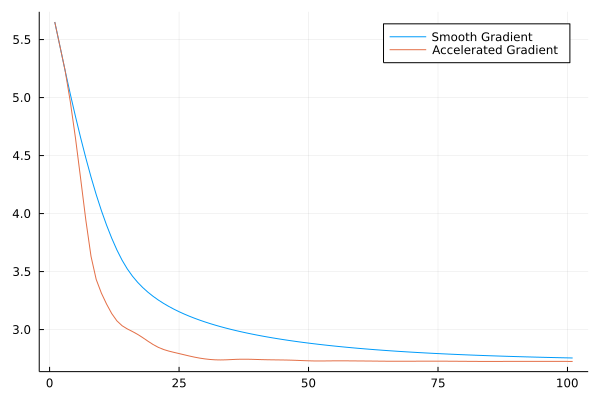
\includegraphics[width=15cm]{objectiveVals.png}
\end{center}
Hi Chatherine, if you need the file for the code and the Julia Project Environment, please contact me I am happy to provide. 
\section*{5.15}
    \subsection*{5.15.1}
        We assume that the $f(x)$ is convex differentiable with minimizer $x^\star$. And we wish to show the following: 
        \begin{align*}\tag{5.15.1.1}\label{eqn:5.15.1.1}
            \text{Gradient Update: } & 
            x_{k + 1} = x_{k} + \lambda_k \nabla f(x_k)
            \\
            \text{Wish to prove: } &
            \frac{1}{2}\Vert x_{k + 1} - x_*\Vert^2 \le 
            \frac{1}{2}\Vert x - x_*\Vert^2 - \gamma_k (f(x_k) - f(x_*)) + 
            \frac{\gamma_k}{2}\Vert \nabla f(x_k)\Vert
        \end{align*}
        To start consider that: 
        \begin{align*}\tag{5.15.1.2}\label{eqn:5.15.1.2}
            \Vert (x_{k + 1} - x_k) - (x_k - x_*)\Vert^2 
            &= 
            \Vert x_{k + 1}\Vert^2 + \Vert x_k - x_*\Vert^2 + 
            2 \langle x_{k + 1} - x_k, x_k - x_*\rangle
            \\
            &= 
            \Vert x - x_*\Vert^2 + \Vert \gamma_k \nabla f(x_k)\Vert^2 
            + 2 \langle \gamma_k \nabla f(x_k), x_k - x_*\rangle
        \end{align*}
        Divides the whole expression by 2 and focuses on the last 2 terms of the expression: 
        \begin{align*}\tag{5.15.1.3}\label{eqn:5.15.1.3}
            & \frac{1}{2}\Vert \gamma_k \nabla f(x_k) \Vert^2 + 
            \langle 
                \gamma_k\nabla f(x_k), x_k - x_*
            \rangle
            \\
            =& \frac{\gamma_k^2}{2}\Vert \nabla f(x_k) \Vert^2 + 
            \gamma_k\langle 
                \nabla f(x_k), x_k - x_*
            \rangle
        \end{align*}
        Using Excercise 4.12 \#4 we have: 
        \begin{align*}\tag{5.15.1.4}\label{eqn:5.15.1.4}
            \langle \nabla f(x_k) - \underbrace{\nabla f(x_*)}_{=0}, x_* - x_k \rangle &\ge 0 
            \\
            f(x_*) - f(x_k) &\ge \langle \nabla f(x_k), x_k - x_*\rangle
        \end{align*}
        Apply \hyperref[eqn:5.15.1.4]{(5.15.1.4)} to \hyperref[eqn:5.15.1.3]{(5.15.1.3)} we have: 
        \begin{align*}\tag{5.15.1.5}\label{eqn:5.15.1.5}
            \frac{\gamma_k^2}{2}\Vert \nabla f(x_k) \Vert^2 + 
            \gamma_k\langle 
                \nabla f(x_k), x_k - x_*
            \rangle
            & \le 
            \frac{\gamma_k^2}{2} \Vert \nabla f(x_k)\Vert^2 + 
            \gamma_k (f(x_*) - f(x_k))
        \end{align*}
        Go back to \hyperref[eqn:5.15.1.2]{(5.15.1.2)} and apply that previous bound we have: 
        \begin{align*}\tag{5.15.1.6}\label{eqn:5.15.1.6}
            \frac{1}{2}\Vert (x_{k + 1} - x_k) - (x_k - x_*)\Vert^2 &= 
            \frac{1}{2}\Vert x - x_*\Vert^2 + \frac{1}{2}\Vert \gamma_k \nabla f(x_k)\Vert^2 
            + \langle \gamma_k \nabla f(x_k), x_k - x_*\rangle
            \\
            &\le 
            \frac{1}{2}\Vert x - x_*\Vert^2+ 
            \frac{\gamma_k^2}{2} \Vert \nabla f(x_k)\Vert^2 + 
            \gamma_k (f(x_*) - f(x_k))
            \\
            &= 
            \frac{1}{2}\Vert x - x_*\Vert^2+ 
            \frac{\gamma_k^2}{2} \Vert \nabla f(x_k)\Vert^2 -
            \gamma_k (f(x_k) - f(x_*))
        \end{align*}
        Which is exactly what we want to show. 
    \subsection*{5.15.2}
        We wish to show that that sequence is minimized by choosing $\gamma_k = (f(x_k) - f^*)/ \Vert \nabla f(x_k)\Vert^2$, where $f^*$ is the minimal value for the function. This is what we wish to prove: 
        $$
            \Vert x_{k + 1} - x^*\Vert^2 \le 
            \Vert x_k - x^*\Vert^2 - 
            \left(
                \frac{f(x_k) - f^*}{\Vert \nabla f(x_k)\Vert}
            \right)^2
        $$
        
        And then proving the the sequence is bounded by: 
        \begin{align*}\tag{5.15.2.1}\label{eqn:5.15.2.1}
            \frac{1}{2}\Vert x_{k + 1} - x_*\Vert^2 &\le 
            \frac{1}{2}\Vert x_k - x_*\Vert^2 - \gamma_k(f(x_k) - f^*) + 
            \frac{\gamma_k^2}{2}\Vert \nabla f(x_k) \Vert^2
            \\
            &=  
            \frac{1}{2}\Vert x_k - x_*\Vert^2 - \gamma_k 
            \left(
                f(x_k) - f^* - \frac{\gamma_k}{2}\Vert \nabla f(x_k)\Vert^2
            \right)
            \\
            \text{Let: }& 
            \partial_{\gamma_k} \left[ 
                \gamma_k(f(x_k) - f^*) + \frac{\gamma^2}{2}\Vert \nabla f(x_k)\Vert^2
            \right]  = 0
            \\
            -(f(x_k) - f^*) + \gamma_k^+ \Vert \nabla f(x_k)\Vert^2 &= 0
            \\
            \gamma_k^+ &= \frac{f(x_k) - f^*}{\Vert \nabla f(x_k)\Vert^2}
        \end{align*}
        Consider the RHS of the first expression in the above block of statements, and substitute the optimal stepside of the expression we have: 
        \begin{align*}\tag{5.15.2.2}\label{eqn:5.15.2.2}
            \Vert x_{k + 1} - x_*\Vert^2 &\le 
            \Vert x_k - x_*\Vert^2 - 2\gamma_k^+(f(x_k) - f^*) + 
            (\gamma_k^+)^2\Vert \nabla f(x_k) \Vert^2
            \\
            &= 
            \Vert x_k  - x_*\Vert^2 - \gamma^+_k(2(f(x_k) - f^*) - \gamma^+ \Vert \nabla f(x_k)\Vert^2)
            \\
            &= 
            \Vert x_k  - x_*\Vert^2 - \gamma^+_k(2(f(x_k) - f^*) - (f(x_k) - f^*))
            \\
            &= \Vert x_k - x_*\Vert - \gamma^+_k(f(x_k) - f^*)
            \\
            &= 
            \Vert x_k - x_*\Vert + 
            \left(\frac{f(x_k) - f^*}{\Vert \nabla f(x_k)\Vert}\right)^2
        \end{align*}
        Which is the statement that we wish to prove. 
    \subsection*{5.15.3}
    In this part we wish to prove that : 
    $$
        f\left(
            \frac{1}{k} \sum_{i = 0}^{k - 1}x_i  
        \right) - f^* \le \frac{2\beta \Vert x_0 - x_*\Vert^2}{k}
    $$
    Inaddition when the function is $\alpha$ strongly convex, wehave the additional results of: 
    $$
        \Vert x_{k + 1} - x_*\Vert^2 \le 
        \left(
            1 - \frac{\alpha}{4\beta}
        \right)
        \Vert x_k - x_*\Vert^2
    $$
    \textbf{Proof}: 
    To make our life easier, we consider using the following notations for the errors and the optimality gap: 
    \begin{align*}\tag{5.15.3.1}\label{eqn:5.15.3.1}
        E_k &= f(x_k) - f^*
        \\
        e_k &= x_k - x^*
    \end{align*}

    Starting with exercise 3.12, the differential characterization for beta smooth function, we have: 
    \begin{align*}\tag{5.15.3.2}\label{eqn:5.15.3.2}
        f(x) + \langle \nabla f(x), y -x\rangle 
        + 
        \frac{1}{2\beta} \Vert \nabla f(x) - \nabla f(y)\Vert^2
        &
        \le f(y)
        \\
        \text{consider: } y&= x_k \quad x = x^* 
        \\
        f^* + \frac{1}{2\beta} \Vert \nabla f(x_k)\Vert^2 &\le f(x_k)
        \\
        \Vert \nabla f(x_k)\Vert^2 &\le 
        2\beta(f(x_k) - f^*) = 2 \beta E_k
        \\
        \implies
        \frac{1}{2\beta} &\le \frac{E_k}{\Vert \nabla f(x_k)\Vert^2}
        \\
        \implies 
        \frac{E_k}{2\beta} &= \frac{E_k^2}{\Vert \nabla f(x_k)\Vert^2}
    \end{align*}
    Then we start with the results from what we proved in \hyperref[eqn:5.15.2.2]{(5.15.2.2)}, And written it as: 
        \begin{align*}\tag{5.15.3.3}\label{eqn:5.15.3.3}
            \Vert e_{k + 1}\Vert^2 
            & \le 
            \Vert e_k\Vert^2 - 
            \left(
                \frac{E_k}{\Vert \nabla f(x_k)\Vert}
            \right)^2
            \\
            \left(
                \frac{E_k}{\Vert \nabla f(x_k)\Vert} 
            \right)^2 &\le 
            \Vert e_{k}\Vert^2 - \Vert e_{k + 1}\Vert^2
            \\\underset{
                \hyperref[eqn:5.15.3.2]{(5.15.3.2)}
            }
            {\implies}
            \frac{E_k}{2\beta}
            &\le 
            \Vert e_{k}\Vert^2 - \Vert e_{k + 1}\Vert^2
        \end{align*}
    Consider summing up the terms in the above inequalities for $0 \le i \le k - 1$:
    \begin{align*}\tag{5.15.3.4}\label{eqn:5.15.3.4}
        \sum_{i = 0}^{k - 1}\frac{E_i}{2\beta}
        & \le 
        \sum_{i = 1}^{k - 1} \Vert e_i\Vert^2 - \Vert e_{i + 1}\Vert^2
        \\
        \frac{1}{k} \sum_{i = 1}^{k - 1}E_i &\le 
        \frac{2\beta}{k} \sum_{i = 1}^{k - 1}\Vert e_i\Vert^2 - \Vert e_{i + 1}\Vert^2
        \\
        \frac{1}{k}\sum_{i = 0}^{k - 1} E_i & \le 
        \frac{2\beta}{k}\left(
            \Vert e_0\Vert^2 - \Vert e_k\Vert^2
        \right)
        \\
        \underset{\text{By Convexity}}{\implies}
        f\left(
            \frac{1}{k}\sum_{i = 0}^{k - 1}E_i 
        \right)- f^*
        &\le
        \frac{2\beta}{k}\left(
            \Vert e_0\Vert^2 - \Vert e_k\Vert^2
        \right) 
        \\
        f\left(
            \frac{1}{k}\sum_{i = 0}^{k - 1}E_i 
        \right)- f^*
        &\le 
        \frac{2\beta}{k}\Vert e_0\Vert^2
        \\
        f\left(
            \frac{1}{k} \sum_{i = 0}^{k - 1}x_i  
        \right) - f^* &\le \frac{2\beta \Vert x_0 - x_*\Vert^2}{k}
    \end{align*} 
    I used telescoping from the second line to the first line in the above block. Just expand the sume and the adjacent terms of the differences will get canceled out. 
    \\[1.1em]
    From the second last line to the last line, we can remove the $-\Vert e_k\Vert^2$ becase it's larger than zero and removing it will make the quantity larger. 
    \\[1.1em]
    Now let's consider the statement from 3.57, the differential characterization of $\alpha$ strongly convex function: 
    \begin{align*}\tag{5.15.3.5}\label{eqn:5.15.3.5}
        f(x_k) - f^* &\ge \frac{\alpha}{2}\Vert x_k - x^*\Vert^2
    \end{align*}
    \begin{align*}\tag{5.15.3.6}\label{eqn:5.15.3.6}
        \Vert \nabla f(x_k)\Vert &= 
        \Vert \nabla f(x_k) - \underbrace{\nabla f(x_*)}_{=0}\Vert \le \beta \Vert x_k - x^*\Vert
    \end{align*}
    Now we may reconsider the results from \hyperref[eqn:5.15.3.4]{(5.15.3.4)}, which is giving us: 
    \begin{align*}\tag{5.15.3.7}\label{eqn:5.15.3.7}
        \Vert x_{k + 1} - x_*\Vert^2 &\le 
        \Vert x_k - x_*\Vert^2 - 
        \left(
            \frac{f(x-k) - f^*}{\Vert \nabla f(x_k)\Vert}
        \right)
        \\
        \Vert x_{k + 1} - x_*\Vert^2 &\le 
        \Vert x_k - x^*\Vert^2 - 
        \left(
            \frac{\frac{\alpha}{2}\Vert x_k - x^*\Vert^2}{
                \beta \Vert x_k - x_*\Vert^2
            }
        \right)
        \\
        &= 
        \left(
            1 - \frac{\alpha^2}{4\beta^2}
        \right)\Vert x_k - x_*\Vert^2
    \end{align*}
    From the first expression to the second one, I replaces the numerator with a smaller quantity, the denominator with a larger quantity, reducing the size of the fraction as whole, and hence reducing the quantity being subtracted smaller, placing an upper bound on the RHS of the first inequality. 
    \\[1.1em]
    That last expression is what we wish to prove for the problem. 
\section*{6.11}
    We were given the accelerated Gradient Descend method which has an interesting sequence that weights on the previous velocity of the descend steps. 
    \subsection*{6.11.1}
        We wish to show that this relation for the sequence holds: 
        \begin{align*}\tag{6.11.1.1}\label{eqn:6.11.1.1}
            \frac{1 - a_{t + 1}}{a^2_{t + 1}} = \frac{1}{a_t^2} \quad
            \forall t \ge 0 
        \end{align*}
        \textbf{Proof}: 
        \begin{align*}\tag{6.11.1.2}\label{eqn:6.11.1.2}
            a_{t + 1} &= \frac{1}{2}
            \left(\sqrt{a_t^4 + 4a_t^2} - a_t^2\right)
            \\
            2a_{t + 1} &= 
            \sqrt{a_t^4 + 4a_t^2} - a_t^2
            \\
            2a_{t + 1} + a_t &= \sqrt{a_t^4 + 4a_t^2}
            \\
            (2a_{t + 1} + a_t^2)^2 &= a_t^4 + 4a_t^2
            \\
            4a_{t + 1}^2 + a_t^4 + 4a_t^2a_{t+1} &= a_t^4 + 4a_t^2
            \\
            4a_{t + 1}^2 + 4a_{t + 1}a_t^2 - 4a_t^2 &= 0
            \\
            a_{t + 1}^2 + a_{t + 1}a_t^2 - a_t^2 &= 0
            \\
            a_{t + 1}^2 + a^2_t(a_{t + 1} - 1) &= 0
            \\
            \frac{1}{a_t^2} + \frac{a_{t + 1} - 1}{a_{t + 1}^2} &= \frac{0}{a_{t}^2a_{t + 1}^2}
            \\
            \frac{a_{t + 1} - 1}{a_{t + 1}^2} &= \frac{1}{a_t^2} \quad \forall t \ge 0
        \end{align*}
    \subsection*{6.11.2}
        We wish to prove that $\sum_{i = 0}^t\frac{1}{a_i} = \frac{1}{a_t^2}$, and then the sequence $a_k$ is upper bounded by the sequence $2/(t + 2)$. 
        \\
        Inductively assume that the statement holds for $n$: 
        \begin{align*}\tag{6.11.2.1}\label{eqn:6.11.2.1}
            \sum_{i = 0}^{t}\frac{1}{a_i} &= \frac{1}{a_t^2}\quad \forall t \le n
        \end{align*}
        \begin{align*}\tag{6.11.2.2}\label{eqn:6.11.2.2}
            \frac{1 - a_{t + 1}}{a^2_{t + 1}} &= \frac{1}{a_t^2}
            \\
            \frac{1}{a^2_{t + 1}} - \frac{1}{a_{t + 1}} &=  \frac{1}{a_t^2}
            \\
            \frac{1}{a_{t + 1}^2} &= \frac{1}{a_t^2} + \frac{1}{a_{t + 1}}
            \\
            \frac{1}{a_{t + 1}^2} &= \sum_{i = 0}^{t}a_i + \frac{1}{a_{t + 1}}
            \\
            \frac{1}{a^2_{t + 1}} &= \sum_{i = 0}^{t+1}\frac{1}{a_{i}}
        \end{align*}
        The statement paramaterized by $n + 1$ holds true. The base case it's not hard to verify, just compute: 
        \begin{align*}\tag{6.11.2.3}\label{eqn:6.11.2.3}
            \frac{1}{a_1} + \frac{1}{a_0} &= \frac{1}{\frac{1}{2}(\sqrt{5} - 1)} +1
            \\
            \frac{1}{a_1^2} &= 
            \frac{1}{\frac{1}{4}(\sqrt{5} - 1)^2}
        \end{align*}
        Which is actually proved by the end of \hyperref[eqn:6.11.1.2]{(6.11.1.2)}. 
        \\
        Next, we wish to prove the upper bound for the sequence. 
        \\[1.1em]
        \par
        This problem is too hard and I can't prove it. I accessed the solutions to multiple peers and they turned out to contain their own algebraic errors. I don't think the upper bound is proven via induction. I do know that the sequence approaches zero monotone. And judging by the amount of efforts I put into this problem, I don't think it's worth it. 
        \par
        Inductively, I used a lot of methods and the fact that the sequence is monotone decreasing. 
        \par
        I gave up after discovering something huge. I try to insert epsilons in inequalities trying to look for additional assumptions can make it better, however, it's futile because all epsilon has to be less than zero, proving that all inductive proof is likely to fail. 
        \par
        Therefore, the proof for the question is not via induction, and it's very likely that this is true. 
        \par
        I computationally verify that the upper bound is extremely tight, and the difference between the sequence $2/(k+2)$ and $a_k$ is a power sequence of power $-2$. The bound is very tight. 
        \par
        Hi Catherine, please check other's algebra on this problem carefully, the proof you went through on Thursday from a student has an algebraic mistake. If you find any legit proof for this problem, please share it via Canvas message to me, I want to know how to handle such a tight bound for this sequence. 
        \par
        Here is the code I used for the numerical investigation of the problem. You will need it to intuitively verify the correct solutions. The code is in matlab. 
        \begin{Verbatim}[numbers=left]
close all;
a = 1;
Points = 0:300;
for Index = Points(2:end)
    p = a(end); % Previous 
    a(end + 1) = (sqrt(p^4 + 4*p^2) - p^2)/2;
end
figure; 
plot(a, '-o', "linewidth", 1); hold on
UpperBound = 2./(Points + 2);
LowerBound = 2./(Points + 3);
plot(UpperBound, "linewidth", 1);
plot(LowerBound, "linewidth", 1);
legend(["sequence", "upper bound", "Lower Bound"])

figure; 
DiffBand = UpperBound - LowerBound; 
loglog(DiffBand);
Coeff = polyfit(log(Points(2:end)), log(DiffBand(2:end)), 1);
disp("Log log Coefficient:")
disp(num2str(Coeff(1)))
        \end{Verbatim}



        


\end{document}
 
